\documentclass{article}
\usepackage[utf8]{inputenc}
\usepackage{appendix}
\usepackage{url}
\usepackage{amssymb}    % for \checkmark
\usepackage{booktabs}  

\title{Scenario Generation for Interactive Urban Environments}
\author{Paritosh Sharma, Hui-Yin Wu}
\date{July 2025}

\usepackage{graphicx}
\usepackage{hyperref}
\usepackage{pgfplots}
\usepackage{tikz}
\usepackage{amsmath}
\usepackage{multirow}
\usepackage{array}
\usepackage{enumitem}
\usepackage{lscape}
\usepackage{geometry} 
\usepackage{adjustbox}

\usetikzlibrary{calc, arrows.meta, positioning, shapes.geometric}

\begin{document}

\maketitle

\section*{Project members}

\begin{itemize}
    \item Scientific team: Paritosh Sharma, Hui-Yin Wu
\end{itemize}

\section{Context and objectives}

The document highlights the work plan for the the WP4 of the ANR Creative 3D~\footnote{\url{https://project.inria.fr/creattive3d/}} project. The expected outcome of this project is to create a generative model that is capable of creating personal
\section{Context and objectives}

The document highlights the work plan for the the WP4 of the ANR Creative 3D~\footnote{\url{https://project.inria.fr/creattive3d/}} project. The expected outcome of this project is to create a generative model that is capable of creating personalized 3D urban traffic scenarios which can be used for conducting simulations in VR.

\section{Introduction}

Virtual Reality (VR) and Augmented Reality (AR) technologies have advanced significantly in recent years, enabling the creation of immersive and interactive environments for various applications. These can be further used to provide personalized training and rehabilitation scenarios. In the context of low vision rehabilitation, these models can be particularly useful to study pedestrian behaviours under normal and simulated vision. However, most simulated environments suffer from perceptual gaps between the designer, the user, and the system. The existing GusT-3D framework~\cite{wu2022designing}, developed during the Creative3D project, provides a foundation to address this. However, the current framework is still limited by its reliance on a fixed set of urban environments and interactions innhibiting its ability to scale.

In parallel, recent works on 3D generative models for urban scenario generation has shown promising results in generating diverse and realistic urban environments. Additionally, these models have been able to capture the diverse nature and the complexities of an urban setting, including the interactions between pedestrians, vehicles, and the environment. Driven by these extraordinary capabilities, exploring the potential of generative models will enable us to create more diverse and realistic urban scenarios.

\section{Related Work}

In this section, we first start by reviewing prior work on scenegraph-guided generation, which is a structured representation of the objects and their relationships within a scene. We then shift our focus existing urban scenario generation models. Finally, we summarize commonly used datasets used for urban scenario generation, and outline validation methods used to assess the quality, diversity, and controllability of the generated scenarios.

\subsection{Scenegraph-guided Generation}

Scenegraph-guided 3D generation is the process of creating 3D environments by leveraging scene graphs, which are structured representations of the objects and their relationships within a scene. A major advantage of scenegraph-guided generation is that it provides a clear relationship between the elements which allows for better generation than other techniques such as simple text prompts or bounding boxes. Scenethesis~\cite{ling2025scenethesis} uses a Vision-Language Model (VLM) to create a scenegraph with parent-child relationships and localizes objects using 3D bounding boxes. Work by Liu et al.~\cite{liu2025controllable} defines scenegraphs as graphs where instance nodes represent countable objects with semantic and positional features, a singleton road node encodes global scene structure, and edges capture both physical proximity among instances and connectivity to the road. X-Scene~\cite{yang2025x} is another work that uses LLMs (Large-Language Models) to create a scenegraph with nodes (objects) and edges (relationships) to facilitate the generation process. Graphdreamer~\cite{gao2024graphdreamer} employs scenegraphs structured around the Visual Genome~\cite{krishna2017visual} format, where nodes represent objects with associated attributes, and edges encode the relationships between these objects to guide the generation process. Despite the advancements in scenegraph-guided generation, all of these works focus on static scenes and do not consider dynamic scenarios where the state of the objects change over time.

\subsection{Diffusion-based 4D Generation}

Diffusion models have emerged as a powerful approach for generating high-quality 3D content by iteratively refining a random noise input into a coherent output. Dreamfusion~\cite{poole2022dreamfusion} initially text-to-3D by optimizing gaussian noise to align with the distribution derived from a text-conditioned diffusion model using Score Distillation Sampling (SDS). This was extended to 4D scenarios in MaV3D~\cite{singer2023text} and 4d-fy~\cite{bahmani20244d}. However, these methods struggle with precise spatial and temporal control of the generated content.

\subsection{Urban Scenario Generation}

This section discusses pre-existing models used for generating scenarios in urban environments. These models can be broadly classified into procedural and deep generative approaches.

\subsubsection{Procedural Methods}

Procedural methods leverage algorithms and rules to generate urban scenarios, often resulting in highly customizable environments. They can be further divided into two categories:

\paragraph{Classic Procedural Generation} use rules or constraints to generate scenes. The most popular procedural approach used for urban scenarios is Scenic~\cite{fremont2019scenic}, which allows users to define scenarios using a probabilistic programming language. Similarly, MetaUrban~\cite{wu2024metaurban} is a popular urban scenario generation framework to create urban micromobility scenarios using the Metadrive~\cite{li2022metadrive} simulator.

\paragraph{LLM-based Procedural Generation} can be used to enhance procedural generation with natural language understanding. For example, ScenicNL~\cite{elmaaroufi2024scenicnl} and ChatScene~\cite{zhang2024chatscene} use LLMs to generate scenic code from prompts and then define the scenarios in Scenic. TTSG\cite{ruan2024traffic} is another framework that uses an to plan a traffic scenario using an LLM in JSON and then render it using CARLA~\cite{dosovitskiy2017carla}. CityX~\cite{zhang2024cityx} is multi-agent framework that uses LLM to assemble assets using the procedural content generation (PCG) library as well as plan actions for the agents in the scenario.

Even though procedural approaches can be highly customizable and allow for precise control over the generated scenarios, they typically suffer from a lack of realism, as they rely on predefined rules that may not capture the full complexity of real-world environments. However, they can be useful in creating diverse scenarios that adhere to specific constraints or requirements. For example, a scenario with a crossroad with a specific number of lanes, a certain type of road surface, and a defined layout of buildings. However, no real crossroad would exist in the world that conforms to these specifications.

\subsubsection{Deep-Generative Methods}

Deep-Generative Approaches have recently become popular for various sorts of 3D generation. To create a complete scenario, some techniques use generative models such as GANs, VAEs or Diffusion models in combination with procedural techniques. These can be broadly classified into the following categories:

\paragraph{Procedural Environments with Deep-Generative Dynamics} generate the static aspects of the environment using procedural techniques, while the dynamic aspects such as vehicles and pedestrians are generated using generative models. For example, Chatdyn~\cite{wei2024chatdyn} uses CARLA~\cite{dosovitskiy2017carla} to construct the traffic environment, then populate it with pedestrians and vehicles, each equipped with an LLM agent to generate a high-level scenario plan. This high-level plan is then executed in a low-level PedExecutor using Text2Motion~\cite{guo2024momask} for pedestrians and VehExectutor using a physics-based, history-aware reinforcement learning controller to produce vehicle trajectories.

\paragraph{Procedural Dynamics with Deep-Generative Environments} generate the dynamic aspects such as vehicles and pedestrians using procedural techniques. UrbanWorld~\cite{shang2024urbanworld} converts 2.5D urban layout data into a structured 3D city with separated assets, applying depth-aware, multi-view diffusion-based texture rendering and UV inpainting to achieve high-fidelity visuals. It also uses an urban MLLM for designing the world and provides dynamic elements which are planned using a random tree path planning algorithm. CityDreamer4D~\cite{xie2024citydreamer} modularly integrates autoregressive token-based generation, neural rendering (e.g., NeRF-style volumetrics), and procedural traffic modeling to synthesize large-scale, time-varying 3D cities.

\paragraph{Complete Deep-Generative Approaches} recreate the static as well as the dynamic aspects using the learnt representation. Infinicube~\cite{lu2024infinicube} constructs a large, dynamic 3D voxel world from input HD maps, vehicle positions, and text prompts; then, it generates photorealistic driving videos and reconstructs the scene into a manipulable 3D environment by fusing voxel- and video-based representations. UniScene~\cite{li2025uniscene} UniScene generates driving scenes in three modalities—semantic occupancy, multi-view video, and LiDAR—by first producing a controllable, temporally consistent occupancy sequence from BEV layouts. This occupancy then serves as unified geometric–semantic guidance to synthesize realistic videos and point clouds, ensuring cross-modal consistency and editability.

\subsection{Datasets}

In this section, we review the datasets that are used to train generative models for road crossing scenarios. Table~\ref{tab:datasets} lists some of the datasets commonly used for training and evaluating generative models in urban environments.

\begin{table}[ht]
\centering
\caption{Overview of selected datasets for foundation model-based scenario generation and analysis.}
\label{tab:datasets}
\renewcommand{\arraystretch}{1.1}
\begin{tabular}{lccccccc}
\toprule
\textbf{Dataset} & \textbf{Year} & \textbf{View} & \textbf{Source} \\
\midrule
SIND~\cite{xu2022drone}             & 2022 & BEV        & Real         \\
Waymo Open~\cite{sun2020scalability}       & 2020 & FPV        & Real  \\
Argoverse~\cite{chang2019argoverse}\cite{wilson2023argoverse}        & 2023 & BEV/FPV    & Real \\
nuScenes~\cite{caesar2020nuscenes}      & 2022 & FPV        & Real \\
KITTI~\cite{geiger2012we}            & 2012 & FPV        & Real \\
Cityscapes~\cite{cordts2016cityscapes}      & 2016 & FPV        & .. \\
HoliCity~\cite{zhou2020holicity}          & 2020 & FPV        & .. \\
OmniCity~\cite{li2023omnicity}          & 2023 & FPV        & ..  \\
GoogleEarth~\cite{xie2024citydreamer}          & 2024 & BEV        & Real  \\
OSM~\cite{xie2024citydreamer}          & 2024 & BEV        & Real \\
CarlaSC~\cite{wilson2022motionsc}          & 2022 & BEV/FPV    & Synthetic \\
CityTopia~\cite{xie2025citydreamer4d}          & 2025 & BEV/FPV    & .. \\
\bottomrule
\end{tabular}
\end{table}

\subsection{Validation}

Table \ref{tab:validation} lists common qualitative and quantitative validation methods used to evaluate the performance of generative models for urban road-crossing scenarios. These methods assess the quality, realism, and diversity of generated scenarios to ensure they fulfill their intended applications and research needs.
\begin{table}[ht]
\centering
\caption{Qualitative and Quantitative Evaluation Methods for Road-Crossing Scenarios}
\resizebox{\textwidth}{!}{
\begin{tabular}{|p{2.5cm}|p{3.5cm}|p{6.2cm}|p{4.5cm}|}
\hline
\textbf{Method Type} & \textbf{Evaluation Approach} & \textbf{Description} & \textbf{Use Case} \\
\hline

\multirow{5}{*}{Qualitative}
& Human Review & Human experts assess realism, scenario diversity, and layout plausibility. & Validates human-perceived quality and applicability of the scene. \\
\cline{2-4}
& Scenario Visualization & 3D visual inspection or rendered videos showing pedestrian, vehicle, and environment interactions. & Helps detect unrealistic or unnatural behavior/configurations. \\
\cline{2-4}
& Surveys & Collects subjective feedback on realism, perceived difficulty, or stress levels from participants. & Measures human-centric realism or emotional response. \\
\cline{2-4}
& Comparison & Compare scenario features (traffic density, gap opportunities, layout) to real-world statistics or distributions. & Validates realism by matching key scenario characteristics to empirical data. \\
\cline{2-4}
& Failure Cases & Identification and analysis of implausible or unsafe scenarios generated by the model. & Guides iterative model improvement. \\
\hline

\multirow{5}{*}{Quantitative}
& Scenario Feature Statistics & Statistical analysis of scenario properties (traffic speed, number/duration of gaps, crosswalk presence, etc.). & Ensures generated scenarios span realistic distributions. \\
\cline{2-4}
& Coverage and Diversity Metrics & Measures distributional entropy or spread of key attributes across all generated scenarios. & Assesses generalizability, scenario variety, and model's exploration of edge cases. \\
\cline{2-4}
& Criticality and Opportunity Metrics & Quantifies the frequency and severity of challenging situations (number of safe gaps, minimum feasible gap size, “no-go” cases). & Evaluates risk/challenge spectrum in the scenario catalog. \\
\cline{2-4}
& Sim2Real Gap (Domain Distance) & Computes metrics like KL-divergence, Earth Mover's Distance, t-SNE or FID/KID between generated and real scenario feature distributions. & Evaluates how closely synthetic scenarios match reality. \\
\cline{2-4}
& Controllability Metrics & Measures how well the model can generate scenarios based on prompts (CLIP, BLIP, VQA, etc.) & Assesses controllability and flexibility of the generative model. \\
\hline

\end{tabular}
}
\label{tab:validation}
\end{table}


%- Forecasting ? (AgentFormer)
%- XDE for agents?

\subsection{Code}

Currently tested code includes:

\subsubsection{Scenic}

Easy to setup and run on colab since the repository is well maintained.

\subsubsection{MagicDrive}

Had issues running due to model size and GPU memory limitations. Also realised only 2D video generation works for now since the code is not uploaded yet for 3D generation.

\subsubsection{MetaUrban/ScenarioNET}

Easy to setup and run since docker container is available and working.

\subsubsection{Threestudio}

Threestudio~\cite{liu2023threestudio} is a collection of 3D generative techniques. Easy to setup and run since docker container is provided. It is well maintained by the community and has a good documentation. Thus, good to test / refer different generative techniques for 3D.

\subsubsection{City Dreamer}

CityDreamer4D~\cite{xie2025citydreamer4d} tried testing the 3D branch with static scenes but encountered issues with the docker container.

\subsubsection{Urban Architect}

Urban Architect~\cite{lu2024urban} - having some dependency issues with pytorch3d. Models too large (~100GB).

\subsubsection{CLIP}

CLIP~\cite{radford2021learning} is a model that can be used to evaluate the quality of generated scenarios. Tested on colab with the pretrained ViT model.

\subsubsection{GraphDreamer}

GraphDreamer~\cite{gao2024graphdreamer} breaks for scenegraph to 3d generation because of GPU memory shortage (surpasses 48 GB). Node level 3d generation works though.

\section{Problem and Open Question}

%To add generative capabilities to frameworks like GusT-3D~\cite{wu2022designing}, have demonstrated the use of scenegraphs and task specifications for pedestrian-in-the-loop simulations. However, these methods are limited in their ability to scale, as they lack generative capabilities needed to produce diverse and realistic scenarios. 
While recent diffusion-based generative models have demonstrated strong capabilities in synthesizing urban scenes from static scenegraphs, they remain limited in their ability to model dynamic urban scenarios. In particular, they struggle to provide precise spatial and temporal control over objects and their interactions, which is essential for simulating realistic traffic and pedestrian behaviors.

This leads to the following open research question:

“How can diffusion models be grounded using scenegraphs to enable controllable generation of urban scenarios that capture both object relationships and their temporal evolution?”

\section{Work Plan}

\subsection{Input Scenegraph}

We represent a temporal (dynamic) scenegraph as a tuple

\begin{equation}
S = (V, E, \mathcal{T}, \tau)
\end{equation}

where

\begin{itemize}
\item $V = \{v_i\}_{i=1}^N$ is a finite set of nodes (objects). Each node $v_i$ is itself a tuple
\begin{equation}
v_i = (\mathrm{id}_i, \mathcal{A}_i, \mathcal{S}_i),
\end{equation}
where
\begin{itemize}
\item $\mathrm{id}_i$ is a unique identifier (string),
\item $\mathcal{A}_i$ is a (possibly sparse) attribute map:
\[
\mathcal{A}_i : \mathcal{K} \rightharpoonup \mathcal{V}
\]
(e.g., color, type, material),
\item $\mathcal{S}_i = \{ (I_{i,k}, \sigma_{i,k}) \}_{k=1}^{K_i}$ is an ordered set of temporal states where each
\[
I_{i,k} = [t_{i,k}^{(0)}, t_{i,k}^{(1)}] \subseteq \mathcal{T}
\]
is a closed time interval and $\sigma_{i,k}$ is a symbolic or structured description of the node's state on that interval (e.g., `accelerates', `stops', or a parametric motion/pose).
\end{itemize}

\item $E \subseteq V \times V$ is a set of directed edges. Each edge $e = (v_i, v_j)$ is augmented by
\begin{equation}
e = (v_i, v_j, r_{ij}, \mathcal{I}_{ij}, \delta_{ij}),
\end{equation}
where
\begin{itemize}
\item $r_{ij}$ is the relation type,
\item $\mathcal{I}_{ij} = \{ J_{ij, \ell} \}_{\ell=1}^{L_{ij}}$ is a set of active time intervals where
\[
J_{ij, \ell} = [\tau^{(0)}, \tau^{(1)}] \subseteq \mathcal{T}
\]
during which the relation holds,
\item $\delta_{ij}$ is an optional descriptive field (string or structured metadata) that further explains the relation (e.g., natural language description or a constraint formula).
\end{itemize}

\item $\mathcal{T}$ is the global time domain. For normalized scenarios, we can take $\mathcal{T} = [0,1]$; for absolute-time scenarios take $\mathcal{T} = [0,T]$ for some duration $T > 0$.

\item $\tau: \bigcup_i \mathcal{S}_i \cup \bigcup_{i,j} \mathcal{I}_{ij} \to \mathcal{P}$ is an optional grounding map from temporal states and relations to parameterized representations (e.g., trajectories, kinematic parameters, animation clips, or low-level simulator actions). $\mathcal{P}$ denotes the space of such parameters.
\end{itemize}

\paragraph{Semantics}
A dynamic scenegraph $S$ encodes both (i) the \emph{static layout} through attribute maps $\mathcal{A}_i$ and relations $r_{ij}$ that are continuously active (or active on $\mathcal{T}$), and (ii) the \emph{dynamic behaviour} through temporal states $\mathcal{S}_i$ and relation active intervals $\mathcal{I}_{ij}$. The grounding $\tau$ maps symbolic descriptions to concrete, simulator-ready parameters.


\subsubsection*{Example}

Figure \ref{fig:scenegraph_example} illustrates the example scenegraph.

\begin{figure}[ht]
\centering
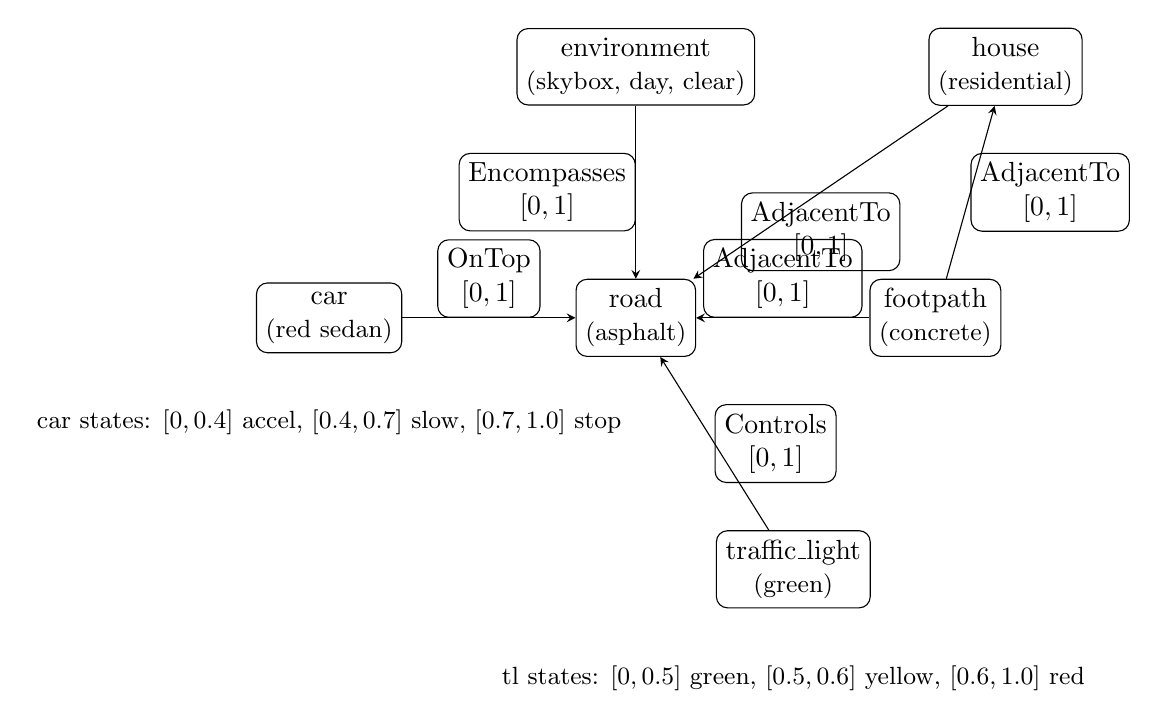
\begin{tikzpicture}[>=stealth, node distance=2.2cm, every node/.style={draw, rounded corners, align=center}]
% Nodes
\node (env) {environment\\\small{(skybox, day, clear)}};
\node (house) [right=of env] {house\\\small{(residential)}};
\node (road) [below=of env] {road\\\small{(asphalt)}};
\node (foot) [right=of road] {footpath\\\small{(concrete)}};
\node (car) [left=of road] {car\\\small{(red sedan)}};
\node (tl) [below=of road, xshift=2.0cm] {traffic\_light\\\small{(green)}};

% Edges
\draw[->] (car) -- node[midway, above]{OnTop\\$[0,1]$} (road);
\draw[->] (tl) -- node[midway, right]{Controls\\$[0,1]$} (road);
\draw[->] (house) -- node[midway, below]{AdjacentTo\\$[0,1]$} (road);
\draw[->] (foot) -- node[midway, above]{AdjacentTo\\$[0,1]$} (road);
\draw[->] (foot) -- node[midway, right]{AdjacentTo\\$[0,1]$} (house);
\draw[->] (env) -- node[midway, left]{Encompasses\\$[0,1]$} (road);

% Temporal annotations (simple)
\node[below=0.6cm of car, draw=none] (car_times) {\small{car states: $[0,0.4]$ accel, $[0.4,0.7]$ slow, $[0.7,1.0]$ stop}};
\node[below=0.6cm of tl, draw=none] (tl_times) {\small{tl states: $[0,0.5]$ green, $[0.5,0.6]$ yellow, $[0.6,1.0]$ red}};
\end{tikzpicture}
\caption{Example dynamic scenegraph (nodes, relations with active intervals, and temporal states).}
\label{fig:scenegraph_example}
\end{figure}


% %input
% example dynamic scenegraph structured

% \begin{tikzpicture}[
%   node distance=5cm and 4cm,
%   box/.style={
%     rectangle, draw, rounded corners, 
%     minimum width=6cm, minimum height=3cm,
%     text width=6cm, align=left, font=\small,
%     fill=gray!10
%   },
%   >={Stealth[length=3mm, width=2mm]}
% ]

% % Nodes
% \node[box] (Pedestrian_1) {
%   \textbf{Pedestrian\_1}\\
%   ontology: Pedestrian\\
%   trajectory: (2,0) $\to$ (4,2)\\
%   speed: 1.2 m/s\\
%   start\_action: Standing\\
%   end\_action: WalkingOffRoad
% };

% \node[box, right=of Pedestrian_1] (Car_1) {
%   \textbf{Car\_1}\\
%   ontology: Car\\
%   trajectory: (0,5) $\to$ (10,5)\\
%   phase1: Stopped until Pedestrian\_1.y $>$ 2\\
%   phase2: Accelerating 0–5 m/s
% };

% \node[box, below=of $(Pedestrian_1)!0.5!(Car_1)$] (Road_1) {
%   \textbf{Road\_1}\\
%   ontology: RoadSegment
% };

% % Edges
% \draw[->] (Pedestrian_1.south) -- (Road_1.north) 
%   node[midway, left, font=\small, align=center] {
%     ontology: CrossesDuring\\
%     (0s–~5s)
%   };

% \draw[->] (Car_1.west) .. controls +(left:2cm) and +(right:2cm) .. (Pedestrian_1.north) 
%   node[midway, right, font=\small, align=center] {
%     ontology: YieldsWhile\\
%     (Pedestrian\_1 in crosswalk)
%   };

% \end{tikzpicture}


% static part
%How to guide the diffusion (variational distillation) using scenegraphs for generating urban scenarios? - Based on the literature and continuing work by Wu et al.~\cite{wu2022designing}, we can use ontological grounding, where we define a scenegraph that captures the relationships between different elements in the scenario, such as pedestrians, vehicles, and the environment. Scenegraph editing for a static scene generation is already shown in works like GraphCanvas3D~\cite{liu2024graph} (\url{https://www.youtube.com/watch?v=4YRTydsv-qg}). The question then is how to use this scenegraph to guide the diffusion process (which mostly uses variational score distillation sampling for text to 3D) for generating dynamic scenarios. % Score distillation for aspects such as terrain, road surface, and other static elements.

% dynamic part
%Predefined assets for pedestrians and vehicles, etc (like MetaUrban)
%How do we create these scenarios allowing for diverse pedestrian behaviors: TODO missing interactions in previous models

% evaluation
%evaluate interactivity, diversity, realism, and controllability (more?) of the generated scenarios?


\section*{Appendix}

\section{Misc}

\subsection{Meeting Notes}

\subsubsection{01/08/2025}    

\begin{itemize}
    \item \textbf{Clarify Image Usage:} Specify what kinds of images are being referred to in the input for the models (e.g., diagrams, real-world photos, layouts).
    
    \item \textbf{Add details on scenegraph:} Provide more information about the scenegraphs (e.g., format, usage, etc.) in the context of the models.
    
    \item \textbf{Avoid Overly High-Level Descriptions:} Some explanations are too abstract.
    
    \item \textbf{Improve Focus on Vocabulary:} Review and refine terminology. Ensure technical or domain-specific terms are clearly defined and used consistently.
    
    \item \textbf{Identify and Specify Missing Interaction Types:} Clearly outline which user/system interactions are missing or underexplored.
    
    \item \textbf{Sharpen Research Question (RQ):} Make the RQ more concrete.
    
    \item \textbf{Better Categorization of Literature:} Reorganize cited papers using clear categories such as research themes, methodologies, etc.
\end{itemize}

\subsubsection{14/08/2025}    

\begin{itemize}
    \item \textbf{RQ still too high level:} Provide more information about the scenegraphs (e.g., format, usage, etc.) in the context of the models.
    
    \item \textbf{Clarify the missing pieces in the SOTA:} 

    \item \textbf{How to address:} diversity -> generative models, realism -> ontology, dynamic -> tasks
    
    \item \textbf{Start with WorkPlan:}     
    
    \item \textbf{Remove relation between GusT-3D and scenegraphs}
\end{itemize}

\subsection{Scenegraph-Controlled Diffusion}

Despite the advancements in urban scenario generation, very few methods have explored the use of scenegraphs to control the generation process. In recent years, the achievements in text-to-image generation has enabled the advancement of text-to-3D generation using Score Distillation Sampling (SDS)~\cite{poole2022dreamfusion} which optimizes a 3D model by aligning 2D images rendered at arbitrary viewpoints with the distribution derived from a text-conditioned diffusion model. Subsequent works including ProlificDreamer~\cite{wang2023prolificdreamer} introduced Variational Score Distillation (VSD) which addresses the over-regularization and mode collapse issues of SDS by introducing a variational formulation that jointly optimizes the 3D representation and a learnable Gaussian noise distribution, enabling more faithful geometry and richer texture generation. GraphDreamer~\cite{gao2024graphdreamer}  uses the the SDS process with scenegraphs to enable more structured and controllable scene generation. However, it uses a simplified static scenegraph representation as shown in Visual genome~\cite{krishna2017visual} in which, nodes represent the objects in the scene, edges represent the relationship between these nodes and attriubtes represent the properties of the node. Example, Elderly (attribute) man (Node) wearing (edge) a hat(node). This limits the ability to generate dynamic scenarios where the relationships between objects change over time.

\subsection{Pedestrian-in-the-Loop}

VR Simulations have been widely used to study pedestrian behavior and interactions in urban scenarios~\cite{wu2018using,tran2021review,mukoya2024jaywalkervr,schneider2020virtually}. This human-in-the-loop approach (also referred as pedestrian-in-the-loop\cite{hartmann2017pedestrian}) allows researchers to collect data on how pedestrians interact with their environment, including their decision-making processes, movement patterns, and responses to various stimuli. These simulations can be used to study a wide range of scenarios, from simple road crossings to complex urban environments with multiple interacting agents. More recently, JaywalkerVR~\cite{mukoya2024jaywalkervr}, a VR human-in-the-loop simulator, used CARLA~\cite{dosovitskiy2017carla} to create four different scenarios: jaywalking, parked cars, four-way stops, and parking lot entrances. The authors created the CARLA-VR dataset by collecting data from 80 participants for these scenarios and used AgentFormer~\cite{yuan2021agentformer}, a trajectory forecasting model for evaluation. Despite the obvious advantages, developing such simulators is still challenging because of the perceptual gaps between the designer, the user and the system as identified by Dourish~\cite{dourish2001action}.

The GUsT-3D framework~\cite{wu2022designing} addresses this by first defining the scene using a scenegraph, which captures the relationships between different elements in the scenario (ontology) and then defining the task to be carried out during the course of the scenario using a GUTasks (intersubjectivity). Lastly, it uses a query component for logging and post-scenario analysis of the experience (intentionality). This framework was also applied by creating a dataset of 6 road-crossing scenarios to study pedestrian behavior under normal and low vision~\cite{wu2023exploring}. Even though GusT-3D framework addresses the perceptual gaps which were identified by Dourish, it still relies on a fixed set of scenarios and interactions.

\subsection{Grounding: Input for Scene Generation}

Generative models have already been applied to urban scenario generation, where models synthesize plausible urban environments, pedestrian layouts, or vehicle positions from various types of input. An input in the context of a generative model is any data—such as a prompt, image, or scenario graph—provided to influence the output. Grounding, on the other hand, is the process of linking elements of that input to specific, coherent representations in the generated scenario, such as ensuring the "footpath" appears visually plausible, is correctly positioned on the "road", and respects spatial relationships or physical constraints. Grounding ensures the generated scenario isn't just randomly composed but meaningfully aligned with the intended semantics of the input. The common ways to do grounding are,

\subsubsection{Rules and Constraints}

\paragraph{Rules} can be used to give a prescriptive logic that defines how to generate or modify a scenario. Rule-based systems are necessarily procedural, meaning they follow a set of predefined steps or algorithms to create scenarios. Table \ref{tab:rule_based_models} lists some of the recent rule-based models for scenario generation. Although these systems allow users to define rules for generating scenarios—such as the placement of buildings, roads, and other elements—they often require an intermediate representation which captures the real-world environments. Creating such representations can be challenging, as it requires a deep understanding of the underlying rules and relationships between different elements. Additionally, rule-based systems can be limited in their ability to generate diverse and realistic scenarios, as they rely on predefined rules that may not capture the full complexity of real-world environments.traffic

\begin{table}[ht]
\centering
    \begin{tabular}{|c|c|c|}
    \hline
    \textbf{Model} & \textbf{Technique} & \textbf{Output} \\ \hline
    CityEngine~\cite{parish2001procedural} & Procedural Modeling with Rules & 3D scene \\ \hline
    Infinigen~\cite{raistrick2023infinite} & Procedural Modeling with Rules & 3D scene \\ \hline
    MetaUrban~\cite{wu2024metaurban} & Description Scripts for Scene Layout & 3D Scenario \\ \hline    
    \end{tabular}
\caption{Rule-based Models for Urban Scenario Generation}
\label{tab:rule_based_models}
\end{table}

\paragraph{Constraints} define conditions that must be satisfied to get a valid scenario. Scenic~\cite{fremont2019scenic} is a probabilistic programming language that allows users to define constraints for generating scenarios. It uses a declarative approach to specify the properties of the scenario, such as the layout, objects, and their relationships. These can then be rendered using a frontend such as CARLA~\cite{dosovitskiy2017carla}. However, it suffers from the same limitations of rule-based systems, as it can only generate scenarios that fit within the defined constraints, potentially missing out on the richness and variability of real-world environments.

\subsubsection{Prompts}

Prompts are textual cues provided to the generative model to guide the scenario creation process. Since the popularity of LLMs like GPT-3, prompts have become a common way to interact with generative models. They can be used to specify the desired characteristics of the scenario, such as the type of environment, objects, and their relationships. Table \ref{tab:prompt_based_models} lists some of the recent prompt-based models for scenario generation.

\begin{table}[h]
\centering
\resizebox{\textwidth}{!}{
    \begin{tabular}{|c|c|c|}
    \hline
    \textbf{Model} & \textbf{Technique} & \textbf{Output} \\ \hline
    ScenicNL~\cite{elmaaroufi2024scenicnl} & Converts LLM Prompts to Scenic Constraints & Scenic Scenario \\ \hline
    ChatScene~\cite{zhang2024chatscene} & Conversational Agent for Scenario Definition using Scenic & Scenic Scenario \\ \hline
    LayoutGPT~\cite{feng2023layoutgpt} & Prompts converted to CSS-like Layout Formatting by LLMs & Layout Representation \\ \hline
    ChatDyn~\cite{wei2024chatdyn} & LLM-based planning and low-level trajectory generation for Pedestrian and Vehicle & 3D Scenario \\ \hline
    Work by Feng et al.~\cite{feng2025text} & JSON to describe layout and 3D models & 3D Scene \\ \hline
    TTSG~\cite{ruan2024traffic} & LLM-based planning and retrieval & 3D Scenario \\ \hline
    3D-SceneDreamer~\cite{zhang20243d} & Prompt to point-of-view image followed by image to 3D & 3D Scene \\ \hline
    GraphCanvas3D~\cite{liu2024graph} & Uses LLM to create a scenegraph and then a 3D scene & 3D Scene \\ \hline
    Scenethesis~\cite{ling2025scenethesis} & Uses LLM to create a scenegraph and then a 3D scene & 3D Scene \\ \hline
    SceneX~\cite{zhou2024scenex} & LLM to plan PCG (Procedural Controllable Generation) & 3D Scene \\ \hline
    Surreal Drivers~\cite{jin2024surrealdriver} & Chain-of-thought prompts & 3D Scene \\ \hline
    Text2nerf~\cite{zhang2024text2nerf} & Text prompts & 3D Scene \\ \hline
    X-Scene~\cite{yang2025x} & Text prompts & 3D Scene \\ \hline
    \end{tabular}
}
\caption{Prompt-based Models for Urban Scenario Generation}
\label{tab:prompt_based_models}
\end{table}

\subsubsection{Layouts}

Layouts are structured representations of scenarios that capture the spatial relationships between different elements, such as buildings, roads, and pedestrians. These may include bird's-eye views, top-down maps, or other forms of spatial representations that provide a high-level overview of the scenario. Table \ref{tab:layout_based_models} lists some of the recent layout-based models for scenario generation.

\begin{table}[ht]
\centering
    \begin{tabular}{|c|c|c|}
    \hline
    \textbf{Model} & \textbf{Technique} & \textbf{Output} \\ \hline
    CC3D~\cite{bahmani2023cc3d} & 2D Layout-based 3D Scene Generation & 3D Scene \\ \hline
    CityDreamer4D~\cite{xie2025citydreamer4d} & Uses a Layout Generator and a traffic scenario generator & 3D Scenario \\ \hline
    Infinicube~\cite{lu2024infinicube} & Text prompts, HD Maps and Bounding Boxes & 3D Scenario \\ \hline
    Work by Zhang et al.~\cite{urbandiff} & BEV map & 3D Scene \\ \hline
    UniScene~\cite{li2025uniscene} & BEV map & Multi-view video \\ \hline
    Savkin et al.~\cite{savkin2021unsupervised} & Scenegraph & Scenario Image \\ \hline
    \end{tabular}
\caption{Layout-based Models for Urban Scenario Generation}
\label{tab:layout_based_models}
\end{table}

\subsubsection{Multimodal}

Multimodal inputs combine different types of data, such as text, images, and structured representations, to provide a richer context for scenario generation. Table \ref{tab:multimodal_models} lists some of the recent multimodal models for scenario generation.

\begin{table}[ht]
\centering
\resizebox{\textwidth}{!}{
    \begin{tabular}{|c|c|c|}
    \hline
    \textbf{Model} & \textbf{Input Type} & \textbf{Output} \\ \hline
    CityX~\cite{zhang2024cityx} & Prompt, OSM file or Semantic Map & 3D Scenario \\ \hline
    CityCraft~\cite{deng2024citycraft} & Layout data and text prompts & 3D Scene \\ \hline
    Work by Liu et al.~\cite{liu2025controllable} & Scenegraph assisted using text prompts & 3D Scene \\ \hline
    GAUDI~\cite{bautista2022gaudi} & Conditioning using prompts or point-of-view images & 3D Scene \\ \hline
    MagicDrive3D~\cite{gao2024magicdrive3d} & Text prompts, Bird Eye View (BEV) map and 3D Bounding Boxes & Reconstructed 3D video \\ \hline
    Scene123~\cite{yang2024scene123} & Text prompt, point-of-view image or Text Description & 3D Scene \\ \hline
    StreetScapes~\cite{deng2024streetscapes} & BEV and height map with support for prompts & Video \\ \hline
    Urban Architect~\cite{lu2024urban} & 3D Layout and Text Prompts & 3D Scene \\ \hline
    Urban World~\cite{shang2024urbanworld} & Layout (generation) and prompts (refinement) & 3D Scenario \\ \hline
    Wonderplay~\cite{li2025wonderplay} & point-of-view image and action (physics) & 3D Video \\ \hline
    \end{tabular}}
\caption{Multimodal Models for Urban Scenario Generation}
\label{tab:multimodal_models}
\end{table}


\bibliographystyle{abbrv}
\bibliography{main}

\end{document}